%%%%%%%%%%%%%%%%%%%%%%%%%%%%%%%%%%%%%%%%%%%%%%%%%%%%%%%%%%%%%%%%%%
%%This presentation was fullly copied from the WSC presentation (dec. 2015)
%% and addapted for the CAA2k16
%% and readdapted as the central stuff  for ICRATES work
%% thus logically  rereadapted for the presentation at TRAC
\documentclass[10pt, notes=show]{beamer}
\usetheme[width=0cm]{Goettingen}
\usecolortheme{rose}
\useoutertheme{default}
\setbeamerfont{caption}{size=\scriptsize}
\setbeamertemplate{navigation symbols}{}
\definecolor{tracblue}{RGB}{4,30,67}
\setbeamercolor{title}{fg=tracblue}
\setbeamercolor{frametitle}{fg=tracblue}
\setbeamercolor{structure}{fg=tracblue}

\addtobeamertemplate{navigation symbols}{}{%
    \usebeamerfont{footline}%
    \usebeamercolor[fg]{footline}%
    \hspace{1em}%
    $\dfrac{\insertframenumber}{\inserttotalframenumber}$
}

\usepackage{fontspec} 
\setsansfont{Futura LT}
%\setmonofont[Scale=0.8]{Monaco} 




%\usepackage{amsmath}
%
%\usepackage{mathptmx}
%\usepackage{latexsym}
\usepackage{graphicx}
\usepackage{mathtools}
%\usepackage{media9}
\usepackage{multimedia}
%\usepackage{multirow}
%\usepackage{caption}
%\usepackage{array}
%\usepackage{listings}
%\usepackage{arydshln}
%\usepackage{multirow}
%\usepackage{ulem}
\usepackage{hyperref}

\DeclarePairedDelimiter\abs{\lvert}{\rvert}%
\DeclarePairedDelimiter\norm{\lVert}{\rVert}%

\title{
    An Agent-Based Model of Trade in the Roman~East~(200~BC--300~AD)
}

\institute{12 April 2018}

\date{\includegraphics[width=.5\textwidth]{./image/TRAC_2018_EDINBURGH_white}}

\author{Simon Carrignon, Tom Brughmans \& Iza Romanowska}


\begin{document}
\begin{frame}
    \maketitle
\end{frame}
\begin{frame}{}
    An Agent-Based Model of Trade in the Roman~East~(200~BC--300~AD):
    \begin{center}
        \parbox{.6\textwidth}{
            \begin{enumerate}
                \item An Agent Based Model: computer models and simulations.
                \item Trade in the Roman East: human activity in past eras. 
            \end{enumerate}
        }
    \end{center}
    How can we use (\textcolor{tracblue}{1}) to learn about (\textcolor{tracblue}{2})?
    \vfill

\end{frame}


\begin{frame}{}
        \textcolor{tracblue}{\large How to know more about something?}
        \vspace{1cm}
    \begin{columns}

        \begin{column}{0.6\linewidth}
            \visible<2->{Claude Bernard style:}
            \begin{itemize}
                \item<3-> Cut in pieces
                \item<4-> Do something
                \item<5-> Repeat
            \end{itemize}
            \visible<6->{Einstein style:}

            \begin{itemize}
                \item<7-> Theories \& laws + Logic \& Maths = New  Theories, new laws, new predictions.
                \item<8-> Wait until someone observe something inline with your predictions 
            \end{itemize}


        \end{column}
        \begin{column}{0.3\linewidth}

            \only<2-5>
            {
                \begin{figure}[h]
                    \centering
                    \includegraphics[width=.5\textwidth]{image/cloclobeber.png}\\
                    {\tiny From: collection BIU Santé Médecine}
                \end{figure}
            }
            \only<6->
            {
                \begin{figure}[h]
                    \centering
                    \fbox{\parbox{\textwidth}{\small image/any-image-with-the-face-of-einstein-choose-the-one-you-prefer.png}}
                    {\tiny From: somewhere in your prefrontal cortex}
                \end{figure}
            }


        \end{column}

    \end{columns}

\end{frame}

\begin{frame}{What if\ldots}
    \begin{itemize}
        \item<+-> Not possible to cut anything.
        \item<+-> No formal theorie nor laws about the studied object.
    \end{itemize}
        \pause
    \begin{figure}[h]
        \centering
        \includegraphics[height=.3\textheight]{image/ghost.jpg}\hfill
        \pause
        \includegraphics[height=.3\textheight]{image/hollow_man_towel.jpg}
    \end{figure}
\end{frame}


\begin{frame}{}
    How to get more informations ?
    \begin{figure}
        \includegraphics[height=.3\textheight]{image/ghost.jpg}\hfill
        \includegraphics[height=.3\textheight]{image/hollow_man_towel.jpg}\\
        \visible<2->{\includegraphics[height=.3\textheight]{image/hollow_man_water.jpg}} \hfill
        \visible<3>{\includegraphics[height=.3\textheight]{image/ghostbusters.jpg}}
    \end{figure}

\end{frame}

\begin{frame}{}
    \center
    Approximate Baeysian Computation\\Linking model and data for an experimental approach to theory.\\
    \vspace{1cm}
    \visible<2->{AKA}\\
    \vspace{1cm}
    \visible<3->{{\huge \bf \textcolor{tracblue}{The Cool Hunters of the Unknown }}}
\end{frame}




\begin{frame}{Hypothetical case}
    \begin{figure}
        \includegraphics[height=.8\textheight]{sagregang/empty.jpg}
    \end{figure}
\end{frame}

\begin{frame}{Limitations}
    \begin{itemize}
        \item<+-> This is not moving
        \item<+-> Impossible to touch or manipulate\ldots
        \item<+-> Some shape can be luckily gathered 
    \end{itemize}
    \vfil
    \begin{figure}
        \visible<+->{\includegraphics[height=.3\textheight]{image/hollow_man_waterNo.jpg} \hfill}
        \visible<+->{\includegraphics[height=.3\textheight]{image/ghostbustersNo.jpg}}
    \end{figure}
\end{frame}

\begin{frame}{Material \& Methods}
    \begin{figure}
        \pause
        \includegraphics[height=.4\textheight]{image/huntersTools.jpg} \\
        \vfill
        \pause
        \includegraphics[width=.4\textwidth]{image/huntersWaiting.jpg} \hfill
        \pause
        \includegraphics[width=.4\textwidth]{image/huntersThrowing.jpg} 
    \end{figure}
\end{frame}

\begin{frame}{Data Gathering \& Data Analysis}
    \begin{figure}
        \only<1>{\includegraphics[height=.8\textheight]{sagregang/empty.jpg}}
        \only<2>{
            Throw and take a pictures\\
            \includegraphics[width=.4\textwidth]{image/huntersWaiting.jpg} \hfill
            \includegraphics[width=.4\textwidth]{image/huntersThrowing.jpg} 
        }
        \only<3>{\includegraphics[height=.8\textheight]{sagregang/shape.jpg}}
        \only<4>{
            Throw again and take a pictures\\
            \includegraphics[width=.4\textwidth]{image/huntersWaiting.jpg} \hfill
            \includegraphics[width=.4\textwidth]{image/huntersThrowing.jpg} 
        }
        \only<5>{\includegraphics[height=.8\textheight]{sagregang/reality_shape.jpg}}
    \end{figure}
\end{frame}

\begin{frame}{Modelling \& Simulation}
    \begin{figure}
        \includegraphics[height=.8\textheight]{sagregang/reality_shape.jpg}
        \hfill
        \includegraphics<+>[height=.8\textheight]{sagregang/bare_model.jpg}
        \includegraphics<+>[height=.8\textheight]{sagregang/model_halfsimu.jpg}
        \includegraphics<+>[height=.8\textheight]{sagregang/model_adjusting.jpg}
        \includegraphics<+>[height=.8\textheight]{sagregang/model_fullsimuHigh.jpg}
        \includegraphics<+>[height=.8\textheight]{sagregang/model_halfsimuLow.jpg}
        \includegraphics<+>[height=.8\textheight]{sagregang/model_fullsimuLow.jpg}
        \includegraphics<+>[height=.8\textheight]{sagregang/model_adjustingB.jpg}
        \includegraphics<+>[height=.8\textheight]{sagregang/model_fullsimuLow+arm.jpg}
    \end{figure}
\end{frame}

\begin{frame}{Modelling \& Simulation}
    \begin{figure}
        \visible<2>{\includegraphics[height=.8\textheight]{sagregang/reality_shape+details.jpg}}
        \hfill
        \visible<1->{\includegraphics[height=.8\textheight]{sagregang/model_fullsimuLow+arm+details.jpg}}
    \end{figure}
\end{frame}

\begin{frame}
    \bf \huge
    And then start the ``real'' hunt.
\end{frame}
\begin{frame}{Our Ghost}
    Roman economic and cultural activity.
    \begin{columns}

        \begin{column}{0.45\linewidth}
            \begin{figure}
                \includegraphics[width=.95\textwidth]{image/roman_market1.jpg}\\
                \parbox{.90\textwidth}{\tiny By JPS68, CC BY-SA 3.0, from Wikimedia Commons}
            \end{figure}
        \end{column}
        \begin{column}{0.45\linewidth}

            \begin{figure}
                \includegraphics[width=0.90\textwidth]{image/roman_market2.jpg}\\
                \parbox{.85\textwidth}{\tiny From: Marisa Ranieri Panetta (ed.): Pompeji. Geschichte, Kunst und Leben in der versunkenen Stadt. p. 146}
            \end{figure}
        \end{column}

    \end{columns}

    \begin{figure}
    \end{figure}
\end{frame}

\begin{frame}{Its shape}

    The ICRATES database:
    \begin{itemize}
        \item presence or absence of 5 types of Sigilata used to produce tableware (bowl, cup, plates)
        \item 178 sites
        \item 500 years (200~BC--300~AD, {\small but will be numbered from 0 to 50 later on})

    \end{itemize}
    \visible<2->{

    \begin{table}
        \centering
        \begin{tabular}{cc}
            Diversity within sites & Distributions among sites \\
            \includegraphics[width=0.4\textwidth]{image/pattern_div.png} &
            \includegraphics[width=0.4\textwidth]{image/pattern_dist.png} \\
        \end{tabular}
    \end{table}
}
\end{frame}

\begin{frame}{The Model}
    \begin{figure}[h]
        \centering
        \includegraphics[width=.8\textwidth]{image/cooev.png}
    \end{figure}
    An agent based model with dynamic processes interacting:
    \begin{itemize}
        \item Cultural activity (people can learn from each other)
        \item Economic activity (people can trade with each other)
    \end{itemize}

\end{frame}

\begin{frame}
    
\end{frame}

\begin{frame}

    One simulation

    \vspace{20pt}

    \only<1>{\href{run:../presentation_script/video_one_simulation_good/output.mpg?autostart&noloop}{\includegraphics[width=0.9\textwidth]{../presentation_script/video_one_simulation_good/one_sim_ex_step-002.png}}}
    \only<2>{\includegraphics[width=0.9\textwidth]{../presentation_script/video_one_simulation_good/one_sim_ex_step-comp.png}}
    \only<3>{\includegraphics[width=0.9\textwidth]{../presentation_script/video_one_simulation_good/one_sim_ex_step-score.png}}
    \only<4>{\includegraphics[width=0.9\textwidth]{../presentation_script/video_one_simulation_good/one_sim_ex_step-check.png}}
    \only<5>{\includegraphics[width=0.9\textwidth]{../presentation_script/video_one_simulation_good/one_sim_ex_step-update.png}}
\end{frame}


\begin{frame}


    An do the same with another simulation %Change good with good1 and bad i

    \vspace{20pt}
    \only<1>{\href{run:../presentation_script/video_one_simulation_good2/output.mpg?autostart&noloop}{\includegraphics[width=0.9\textwidth]{../presentation_script/video_one_simulation_good2/one_sim_ex_step-002.png}}}
    \only<2>{\includegraphics[width=0.9\textwidth]{../presentation_script/video_one_simulation_good2/one_sim_ex_step-comp.png}}
    \only<3>{\includegraphics[width=0.9\textwidth]{../presentation_script/video_one_simulation_good2/one_sim_ex_step-score.png}}
    \only<4>{\includegraphics[width=0.9\textwidth]{../presentation_script/video_one_simulation_good2/one_sim_ex_step-check.png}}
    \only<5>{\includegraphics[width=0.9\textwidth]{../presentation_script/video_one_simulation_good2/one_sim_ex_step-update.png}}

\end{frame}


\begin{frame}


    And another\ldots %Change good with good1 and bad i

    \vspace{20pt}
    \only<1>{\href{run:../presentation_script/video_one_simulation_good3/output.mpg?autostart&noloop}{\includegraphics[width=0.9\textwidth]{../presentation_script/video_one_simulation_good3/one_sim_ex_step-002.png}}}
    \only<2>{\includegraphics[width=0.9\textwidth]{../presentation_script/video_one_simulation_good3/one_sim_ex_step-comp.png}}
    \only<3>{\includegraphics[width=0.9\textwidth]{../presentation_script/video_one_simulation_good3/one_sim_ex_step-score.png}}
    \only<4>{\includegraphics[width=0.9\textwidth]{../presentation_script/video_one_simulation_good3/one_sim_ex_step-check.png}}
    \only<5>{\includegraphics[width=0.9\textwidth]{../presentation_script/video_one_simulation_good3/one_sim_ex_step-update.png}}

\end{frame}

\begin{frame}


    Until you have enough

    \vspace{20pt}
    \only<1>{ \href{run:../presentation_script/full_video_epsilon_0.15/output1.mpg?autostart&noloop}{\includegraphics[width=0.9\textwidth]{../presentation_script/full_video_epsilon_0.15/all_sim_frame-00094.png}}  }
    \only<2>{ \href{run:../presentation_script/full_video_epsilon_0.15/output2.mpg?autostart&noloop}{\includegraphics[width=0.9\textwidth]{../presentation_script/full_video_epsilon_0.15/all_sim_frame-00640.png}}  }

\end{frame}

\begin{frame}

    And repeat the same but being more restrictive:
    \vspace{20pt}
    \only<1>{ \href{run:../presentation_script/full_video_epsilon_0.012/output1.mpg?autostart&noloop}{\includegraphics[width=0.9\textwidth]{../presentation_script/full_video_epsilon_0.15/all_sim_frame-00094.png}}  }
    \only<2>{ \href{run:../presentation_script/full_video_epsilon_0.012/output2.mpg?autostart&noloop}{\includegraphics[width=0.9\textwidth]{../presentation_script/full_video_epsilon_0.15/all_sim_frame-00640.png}}  }

\end{frame}

\begin{frame}
    \centering
    \includegraphics[width=0.8\textwidth]{image/result_abc_best.png}
\end{frame}

\begin{frame}{Hypothesis Testing}
    What if we change some of the elements of the model?
    \begin{itemize}
        \item Copy the bests $\rightarrow$ Random copy 
    \end{itemize}
\end{frame}

\begin{frame}
    \centering
    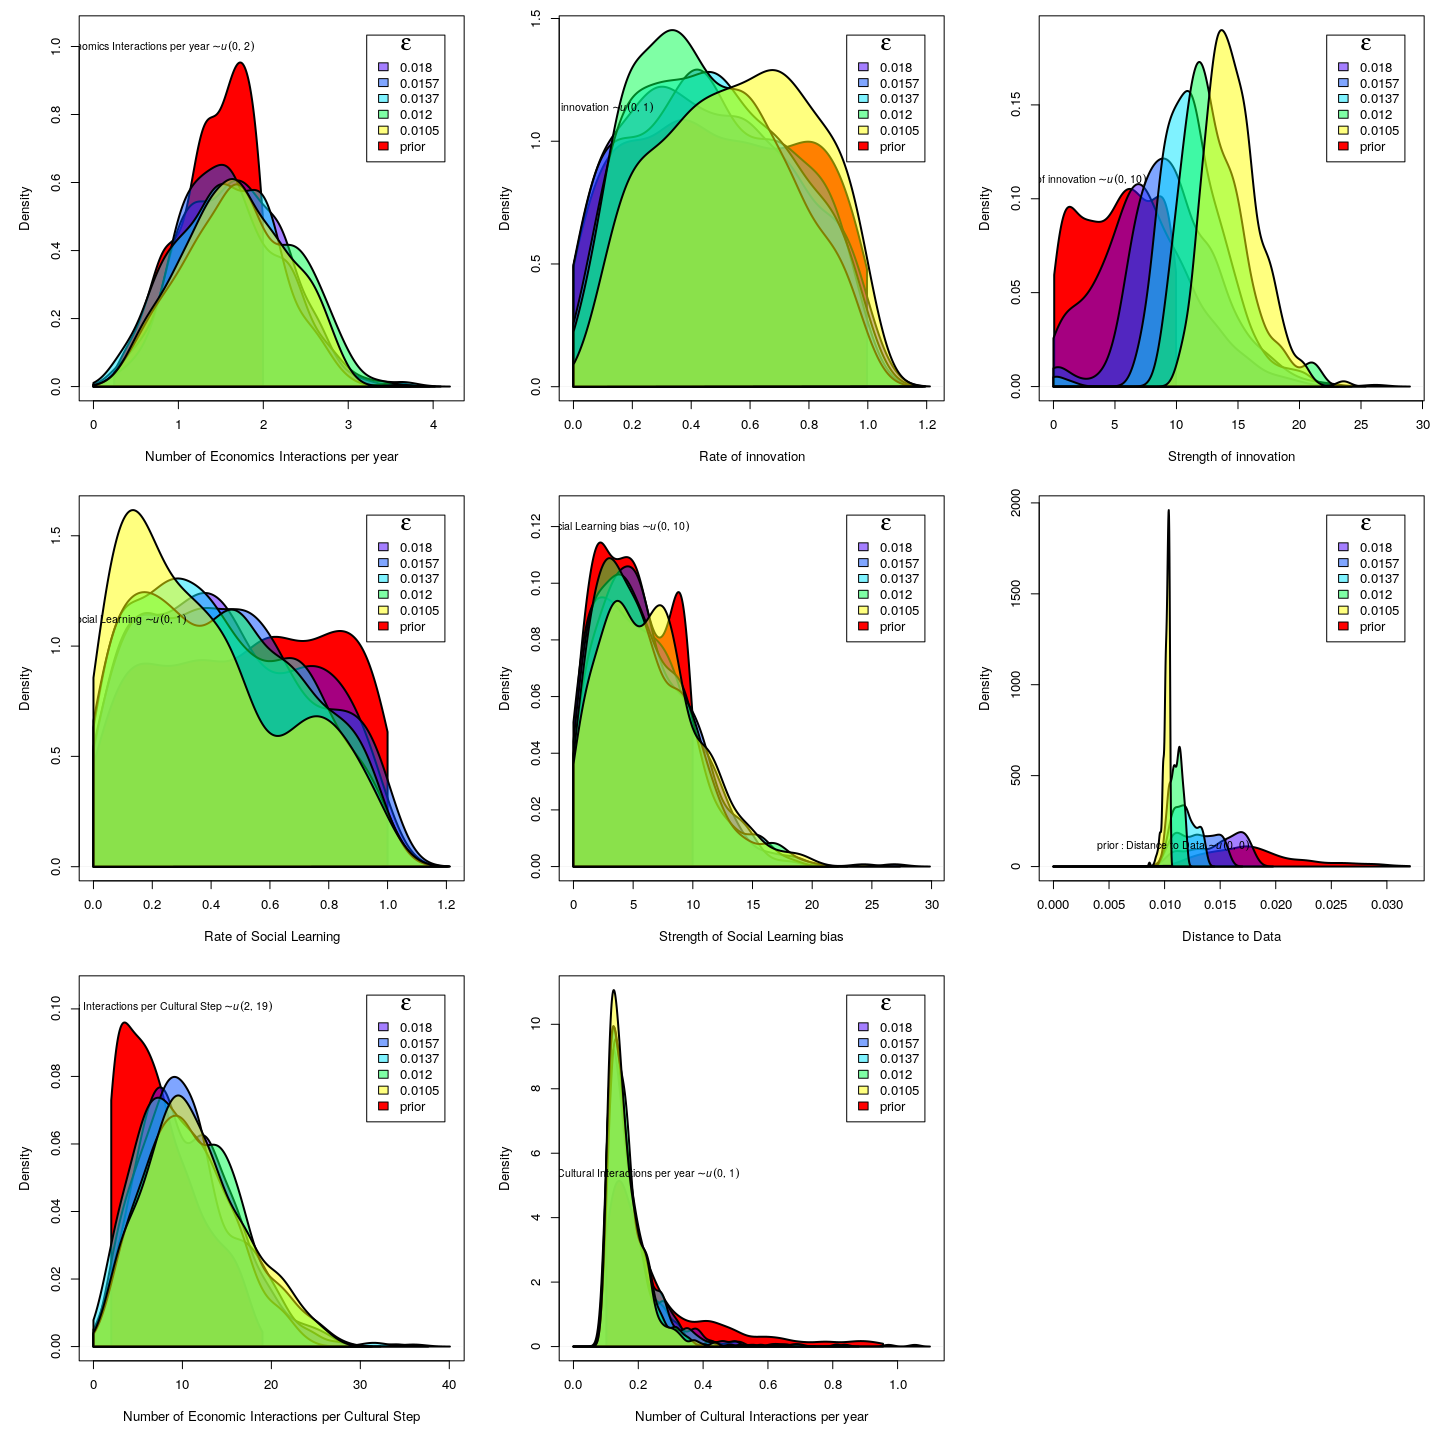
\includegraphics[height=0.95\textheight]{image/result_abc_rand.png}
\end{frame}

\begin{frame}{Hypothesis Testing}
    \begin{columns}

        \begin{column}{0.6\linewidth}
    Compare results for the more restrictive epsilons:
    \begin{itemize}
        \item<+-> How many simulations needed? 
            \begin{itemize}
                \item<+-> Relatively similar for both ($\approx 30\,000$)
            \end{itemize}
        \item<+-> Compare parameters by parameters
    \end{itemize}
        \end{column}
        \begin{column}{0.45\linewidth}
    \begin{figure}
        \includegraphics[height=0.8\textheight]{image/random_vs_bestbias.png}
    \end{figure}

        \end{column}

    \end{columns}
\end{frame}

\begin{frame}
    Approximate Bayesian Computation allows to link data to models by giving us the probability of one model to reproduce observed patterns.
    \begin{itemize}
        \item<+-> Flexible,
        \item<+-> Few assumptions needed (neither on data nor model side),
        \item<+-> Heavy computational cost,
        \item<+-> Central role of transdisciplinarity (central role interpretation and expert knowledge). No strict answer ($<.05 \rightarrow$ OK,$>.05 \rightarrow$ not OK).
    \end{itemize}
    
\end{frame}

\begin{frame}
	\begin{center}
		\includegraphics[width=2cm]{image/LOGO-ERC.jpg} \hfil	\includegraphics[width=3cm]{image/epnetLogo.png}\\
		\includegraphics[width=3cm]{image/leverhulme}\\
		\vspace{.5cm}
		Thank you for you attention\\
		\vspace{.5cm}
		\scriptsize
			http://www.roman-ep.net/\\
			@simoncarrignon\\
		\vspace{.5cm}
		\includegraphics[width=4cm]{image/bscLogo}\\
	\end{center}


\end{frame}

\end{document}

